\setstretch{1.6}
\sectiontitle{6}{Tip Tracking Integration}
\lhead{Tip Tracking Integration} % section header
As mentioned in the project context an algorithm for capturing and processing the images from the cameras has already been developed by a previous student. This code was written in python and its aim was to deduce the position and direction of the tip of the ribbon while it moves in the brain phantom effectively "Tip Tracking". However, this code had not been developed for real-time use, but rather post-processing of videos.  Therefore it had to be refactored and somewhat rewritten for this project. Since the tip data acquired by this algorithm was then to be used in the closed-loop path following control system, it was also necessary to develop a method of sharing this data in real time with the C++ control system developed in Qt. This section therefore details the refactoring and communication implementation necessary to allow for live vision-feedback.

\lhead{Tip Tracking Integration - Theory} % section header
\subsection{Theory}
\subsubsection{Types of Communication Protocols}
There are several ways to establish a communication layer that allows real-time data transfer between two programs, often referred to as InterProcess Communication (IPC). Below is a brief analysis of each relevant method.


\paragraph*{File-based communication}
The simplest solution in terms of implementation is file based communication. One system would for each data point write to a file which is subsequently read by the receiving system. This requires the receiving system to continuously monitor the file for updates introducing latency that is further exacerbated by file system access times and disk I/O overhead. 

In terms of fault tolerance, file-based communication has the benefit of data persisting even if a process crashes, however it is not designed for high-frequency updates \cite{gray_interprocess_2003}. Race conditions can occur if both the vision and control systems attempt to access the file simultaneously. Locking mechanisms can mitigate this, but at the cost of further increasing latency \cite{gray_interprocess_2003}. 

\paragraph*{Shared memory}
A significantly faster method is shared memory. Shared memory allows multiple processes to access a common memory space, enables rapid data exchange without the overhead of disk I/O or network communication. However it also introduces concurrency and data consistency challenges. \cite{gray_interprocess_2003}

Since multiple processes may attempt to read and write simultaneously, synchronization mechanisms such as mutexes or semaphores are required to prevent race conditions \cite{burns_real-time_2009}. This adds complexity and thus makes the system less robust and maintainable. Another challenge is that shared memory must be allocated and managed by both processes. This makes it difficult to integrate across different programming languages where data structures may not be inherently compatible. Thus the complexity, lack of language compatibility and make it impractical for this application.

\paragraph*{Named Pipes}
Named Pipes allow data to be transmitted between processes on the same machine asynchronously by operating as a first-in, first-out (FIFO) buffer \cite{gray_interprocess_2003}. Compared to file-based communication, pipes offer lower latency and are more efficient for continuous data streaming \cite{gray_interprocess_2003}. The main limitation in the context of this project is that they are constrained to a single machine. This limits the scalability since in a later revision one might want to run the vision and control systems on separate machines in a distributed setup. 

\paragraph*{Message queues}
Message queues provide structured message passing using a queue-based architecture \cite{kleppmann_designing_2017}. Systems such as RabbitMQ and Apache Kafka provide reliable message delivery making message queues highly fault tolerant. However they also introduce latency due to message buffering and broker management \cite{kleppmann_designing_2017}. Meaning that they may not be ideal for real-time application such as this onw where low-latency streaming is of a higher priority than durable message queueing.

\paragraph*{Networking (Sockets and ZeroMQ)}
Networking-based communication, using either raw sockets or messaging libraries such as ZeroMQ \cite{noauthor_zeromq_nodate}, provides a flexible and scalable solution \cite{lauener_how_2018}. Raw sockets allow direct communication over a network using protocols such as TCP or UDP. TCP ensures reliable message delivery but introduces additional latency. The choice between TCP and UDP is a trade-off between reliability and variability of delays: UDP does not perform flow control and does not retransmit lost packets, so it avoids some of the resasons for variable network delays \cite{kleppmann_designing_2017}. Unlike TCP, UDP does not guarantee message delivery, meaning that packets may be lost.  However, for real-time control, receiving the most recent data is more important than ensuring that every packet arrives. Since the vision data is used as feedback, occasional packet loss is preferable to the latency caused by TCP retransmissions. 

ZeroMQ provides a higher-level abstraction for message-based communication and offers built-in support for various messaging patterns, including publish/subscribe (pub/sub), request/reply and push/pull \cite{lauener_how_2018}. The pub/sub model is especially advantageous system since it enables efficient real-time streaming of data to multiple subscribers with minimal overhead. 


\lhead{Tip Tracking Integration - Methods} % section header
\subsection{Methods}

\subsubsection{Vision Code Refactoring Methodology}
As mentioned, there was an existing Python-based 3D tip tracking algorithm. However, it was implemented in a single file and hand not been developed for real-time use. Meaning that it did not have the structure necessary to allow for simple alterations that would transform it into real-time detection system. The system also needed additional implemented functionality such as image capturing and communication to the Qt-based control system. Therefore it was decided that the code had to be restructured and altered. This was done according to the same code quality criteria discussed in the theory section in the Software Refactoring chapter.
\newline \newline
Additionally to make it suitable for real-time feedback it was necessary to thread the system. This is due to the original systems reliance on YOLO \cite{redmon_you_2016}, a deep learning-based object detection algorithm, which is too computationally heavy for non-threaded real-time use.

\subsubsection{Switching to 2D Tip Tracking}
As the project progressed it became clear that even after refactoring the 3D vision system did not perform well enough for real-time vision. This was due to the slow computationally heavy step of running each frame through YOLO which limited the system significantly, even after assigning it to its own thread. There were also other issues, such as the system having been trained previously on images where the ribbon was moving in a agarose brain phantom. Since 5\% bovine gelatin was used in this project instead due to it having closer mechanical properties to the brain, the detection turned out to be quite poor. This led to jumps in the systems estimation of the tip position and direction and, at times, no detection at all.
\todo{picture of ribbon in agarose vs gelatin?}
\newline \newline
Therefore Lorenzo Noseda developed a 2D version that instead utilizes classical thresholding and skeletonization of the images and thereby extracts the 2D tip position and direction. A new version of the refactored real-time 3D tip tracking was thereafter developed for this thesis, where the 2D tip detection was inserted into the structure instead of the 3D YOLO detection.

\subsubsection{Choosing a Communication Protocol}
In order to establish a robust connection between the already existing Python-based tip tracking system and the C++/Qt-based control system several ways of establishing an interface were evaluated. In order to choose the most suited communication method a set of evaluation criteria based on their suitability for real-time dat streaming \textit{Designing Data Intensive Applications} \cite{kleppmann_designing_2017} were used.

\begin{enumerate}
    \item \textbf{Latency and Real-Time Performance} - The ability to provide low-latency communication suitable for real-time control.
    \item \textbf{Fault Tolerance and Robustness} - Resiliance to failures such as dropped messages or system crashes.
    \item \textbf{Communication Model} - Suitability for push-based (streaming) or pull.based (request-response) communication
    \item \textbf{Ordering and Consitency Guarantees} - The ability to ensure data arrives in the correct order.
    \item \textbf{Scalability} - The capability to accommodate future system expansions, such as integrating communication with a potential real-time path planning algorithm.
    \item \textbf{Ease of Implementation and Maintenance} - Complexity of integrating the communication method into the existing system.
\end{enumerate}




\lhead{Tip Tracking Integration - Design} % section header
\subsection{Design}
\subsubsection{Choice of Communication Protocol}
The methods discussed in the theory section were all considered for enabling communication. File-based communication was ruled out early due to high latency and non-robust performance. Shared memory and named pipes offer better performance but had limited scalability and poor cross-platform/language compatibility. Message queues were also excluded as their high reliability and fault tolerance came at the cost of increased latency.
\newline \newline 
ZeroMQ was selected because it offers a lightweight, high-performance messaging layer with built in support for communication patterns such as publish/subscribe and request/reply \cite{lauener_how_2018}. The pub/sub pattern is especially useful here, as it allows the vision system to breadcast real-time data to the control system. This may also be easily expanded later one so that for example a real-time path planning algorithm can simply subscribe to the vision data.
\newline \newline
To further reduce latency, ZeroMQ was configured to use UDP instead of TCP in order to avoid delays caused by retransmission. Making it more suitible for real-time feedback where receiving the most recent data is the priority. 



\lhead{Tip Tracking Integration - Results} % section header
\subsection{Results}

\subsubsection{Final Refactored Vision System}
The final refactored system consists of five primary modules as shown in figure \ref{fig:visioncode}, each with clearly defined responsibilities. A description of each class can and a sequence diagram that illustrates the real-time processing flow can also be found in the appendix.

\begin{figure} [H]
    \centering
    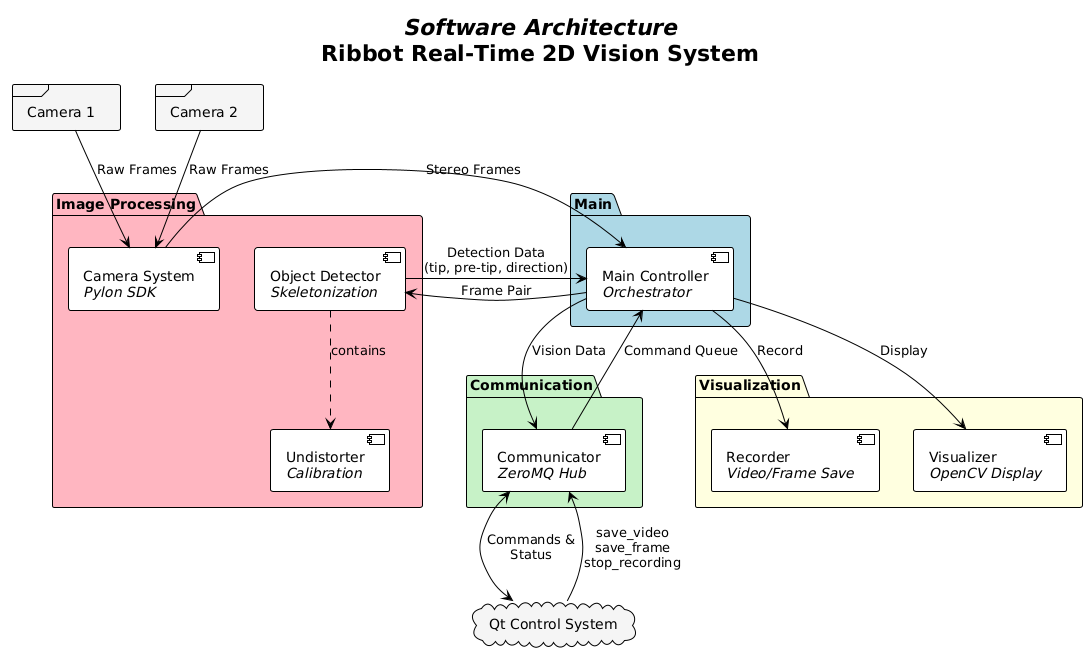
\includegraphics[width=\linewidth]{images/Software documentation/visionmodules.png}
    \caption{Modular architecture of the refactored vision system}
    \label{fig:visioncode}
\end{figure}

The vision system captures synchronized video streams from the Basler cameras at 10FPS.  The detection pipeline developed by Lorenzo employs reference frame computation, morphological operations for noise reduction and iterative thinning algorithms to extract the centerline. This allows it to detect the tip position and reference point approximately 1mm proximal to the tip.A normalized direction vector is then computed based on these points. The coordinates, along with a normalized vector are formatted into a structure message which is then processed and sent by the communication class.

\todo{figure of skeletonized ribbon?}

In terms of threading the \texttt{ObjectDetector} and \texttt{CameraSystem} classes implement dedicated worker threads with queue-based frame management. Frame queues use a latest-frame-only strategy to maintain low latency in case of varying processing time.

\todo{figure of vision system detections}


\subsubsection{Communication protocol between Python and Qt}
In the final communication system the Python based vision system acts as a pyblisher and continuously streams messages containing the timestamp, the two-dimensional coordinates of the detected tip and a point 1mm procimal to the tip, as well as a normalized direction vector. 
\begin{figure} [H]
    \centering
    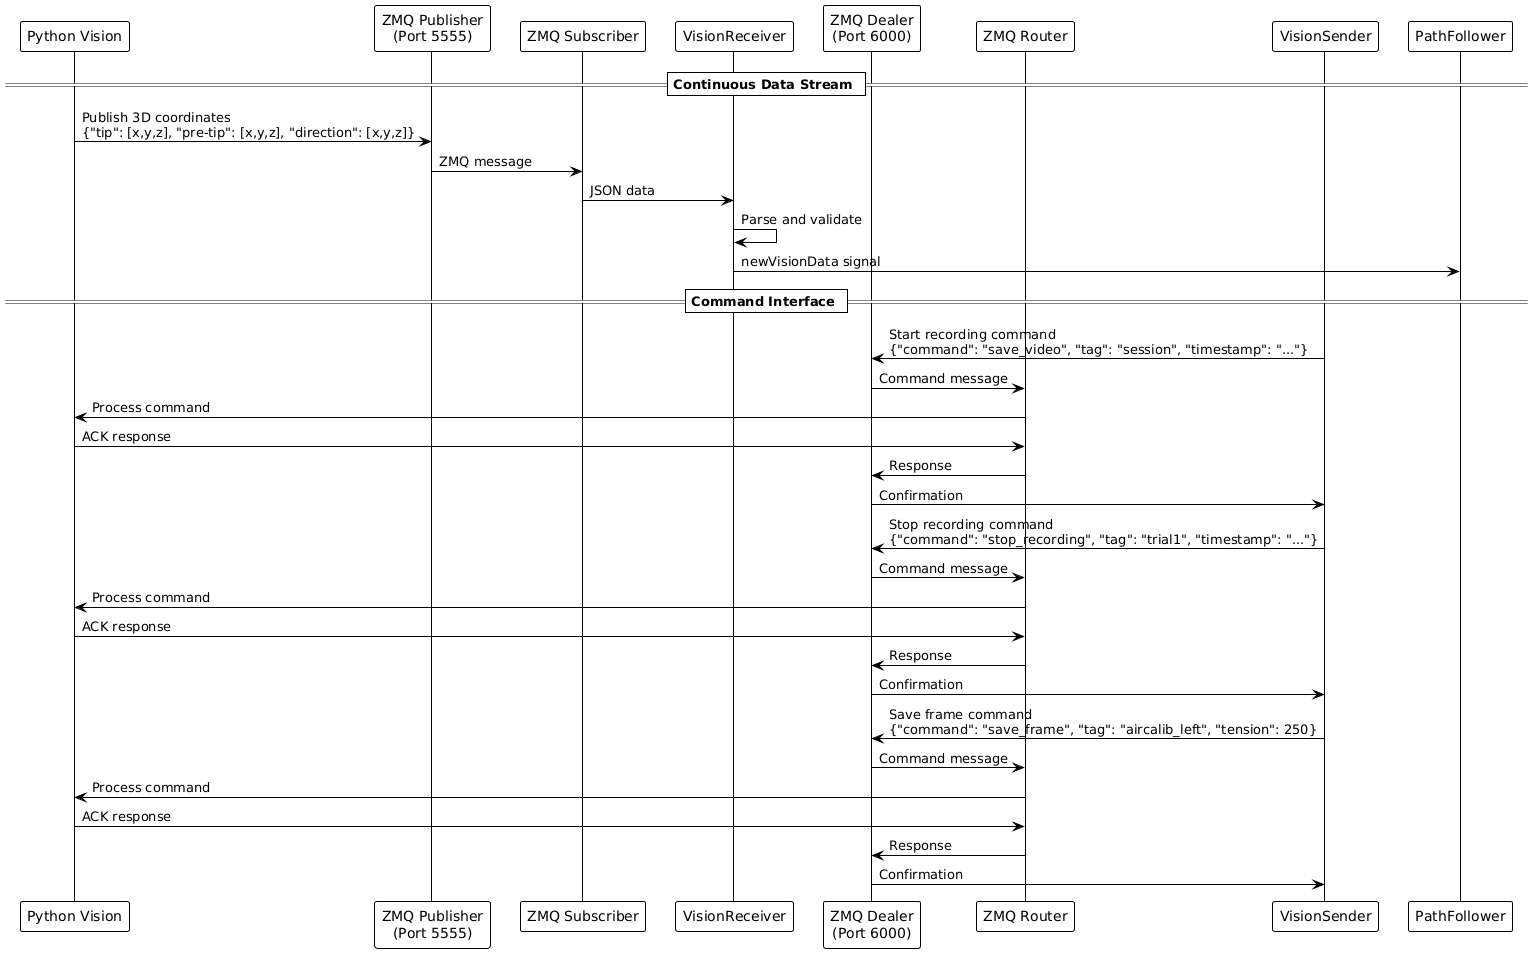
\includegraphics[width=1.1\linewidth]{images/Software documentation/visionSequencediag.png}
    \caption{Sequence diagram of the communication between python vision system and Qt control system}
    \label{fig:seqComm}
\end{figure}


\newline \newline 
Before transimission, the coordinates are transformed from the vision system's coordinate frame to that used by the control system. The Qt based control system includes a dedicated subscriber thread that listens for updates on the specified ZeroMQ address. Once a message is received, the thread extracts the relevant information and updats the path following system with the latest tip and direction data. 
\newline \newline
In addition to receiving data, the control system can also send commands to the vision module using a separate ZeroMQ DEALER socket. Three commands are currently implemented: \texttt{save\_video}, which start recording video frames with an optional session tag; \texttt{stop\_recording}, which terminates the ongoing recording session; and \texttt{save\_frame}, which captures and stores a single image frame annotated with metadata. These commands allow the contro system to trigger frame captures and recordings in sync with contrl events and to annotate them with relevant metadata. This enables accurate offline analysis and alignment of visual and control data logs.



\subsection{Discussion}
This implementation is scalable in the sense that if you want to implement on-line path calculation based on the vision data it can simply also just subscribe to the vision data.

The fact that any subscriber on vision network can receive updates. This ensures flexivbility and allows additional components such as logging or monitoring tools or real time path planning to be added as subscribers in the future.

By leveraging low-latency, connectionless messaging, the system ensures that the most recent vision data is always available without the delays associated with TCP retransmissions or message queues. The pub/sub model further enhances scalability, allowing additional subscribers to be integrated as needed.

By structuring the vision and control system communication in this manner, the system achieves fast, robust, and scalable data exchange while maintaining the flexibility to accommodate future improvements. The combination of efficient data serialization, independent processing threads, and network optimizations ensures that the communication layer operates at a high frequency without compromising the responsiveness of the control system. 

 This combination—ZeroMQ over UDP—provides a fast, scalable, and maintainable communication layer ideal for streaming real-time vision data to the control system.

\todo{rewrite whole subsubsection}
